\section*{Datentypen}
\subsection*{Bite}
\subsubsection*{2er Potenzen}
\begin{center}

\resizebox{\columnwidth}{!}{%
\begin{tabular}{|c|c|c|c|c|c|c|c|c|c|c|}
\hline
2${}^{10}$ & 2${}^{9}$ & 2${}^{8}$ & 2${}^{7}$ & 2${}^{6}$ & 2${}^{5}$ & 2${}^{4}$ & 2${}^{3}$ & 2${}^{2}$ & 2${}^{1}$ & 2${}^{0}$ \\ \hline
1024 & 512 & 256 & 128 & 64 & 32 & 16 & 8 & 4 & 2 & 1 \\ 
\hline
\end{tabular}}
\end{center}

\begin{center}
\resizebox{\columnwidth}{!}{%
\begin{tabular}{|c|c|c|c|c|c|c|c|c|}
\hline
2${}^{0}$ & 2${}^{-1}$ & 2${}^{-2}$ & 2${}^{-3}$ & 2${}^{-4}$ & 2${}^{-5}$ & 2${}^{-6}$ & 2${}^{-7}$ & 2${}^{-8}$ \\ \hline
1 & 0.5 & 0.25 & 0.125 & 0.0625 & 0.03125 & 0.015625 & 0.0078125 & 0.00390625 \\ 
\hline
\end{tabular}}
\end{center}
\subsection*{Bitshift}
$>>$ Right Shift signed (mit 1en auffüllen)\\
$>>>$ Right Shift unsigned (mit 0en auffüllen)\\
$<<$ Left Shift unsigned (mit 0en auffüllen)
\subsection*{Float}
\subsubsection*{Floating Point nach Dezimalzahl}
\begin{center}
\resizebox{\columnwidth}{!}{%
\begin{tabular}{|c|c|c|c|c|c|c|c|c|c|c|c|c|c|c|c|c|}
V & \multicolumn{8}{c|}{Exponent 8 Bit} & \multicolumn{8}{c|}{Mantisse} \\ \hline
1 & 1 & 0 & 0 & 0 & 0 & 1 & 0 & 1 & 0 & 0 & 1 & 0 & 0 & 1 & 0 & ... \\ \hline
\end{tabular}}
\end{center}

V = \textbf{-1}

Exponent = 128 + 4 + 1 = 133 => 133 - 127 (Bias) = \textbf{6}

1.0010010 => Komma um 6 Stellen nach Rechts verschieben
1001001.0 = \textbf{73}

\subsubsection*{Dezimalzahl nach Floating Point}

-23.5
\begin{itemize}
\item[1.] Dezimal zu Binär: 00010111.1
\item[2.] Normalisieren: 00010111.1 => 0001.011110...
\item[3.] Exponent: 4 + 127 (Bias) = 131 => 1000 0011
\end{itemize}
\subsection*{Oktal zu Binär}
\begin{center}
	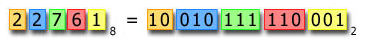
\includegraphics[width=10cm]{images/oktbin}
\end{center}